%%%%%%%%%%%%%%%%%%%%%%%%%%%%%%%%%%%%%%%%%%%%%%%%%%%%%%%%%%%%%%%%%%% 
%                                                                 %
%                            CHAPTER FOUR                         %
%                                                                 %
%%%%%%%%%%%%%%%%%%%%%%%%%%%%%%%%%%%%%%%%%%%%%%%%%%%%%%%%%%%%%%%%%%% 
 
\chapter{Molecular Dynamics Simulations of Clay-Water Interfaces}

	\section{Theoretical Background}
		Molecular dynamics simulations of the clay-water interface were performed to further investigate the experimentally observed trends in the behavior of the vibrational modes of the water molecules, and the pH of the system as seen in chapter three. Computational methods considering the classical and basic quantum mechanical effects have previously been developed and implemented in mature codes. The basic theory of these methods, and the setup of the simulated system are provided here. 
	
		
		\subsection{Traditional Force Field Approximations}
			The more traditional approach to molecular dynamics is to approximate the basic forces which act on atoms and molecules with well known and accepted functions to approximate such behaviors. The first source one must consider is the electrostatic force between atoms which are charged, or approximated as having a charge, which is modeled using the form of the Coulomb potential between two point charges:
			\begin{equation}
				U_{C_{ij}} = k_e \frac{q_iq_j}{r_{ij}}
				\label{eq:coulomb}
			\end{equation}
			where $k_e$ is the Coulomb constant. 
			
			The next force considered is the van der Waals force, between atoms in different molecules. Two common methods exist for approximating this force, being either the 12-6 or the 9-6 Lennard-Jones (LJ) potentials. In this work, we shall only make use of the 12-6 LJ potential, as this is the form used in the consistent valence force field (CVFF), which will be used in the subsequent simulations \cite{heinz2005force}. We arrive at a function describing these interactions of the form
			\begin{equation}
				U_{LJ_{ij}} = 4\epsilon_{ij}\bigg[ \bigg(\frac{\sigma_{ij}}{r_{ij}}\bigg)^{12} - \bigg(\frac{\sigma_{ij}}{r_{ij}}\bigg)^6\,\bigg]
				\label{eq:lj}
			\end{equation}
			with $\epsilon_{ij}$ being the depth of the potential well and $\sigma_{ij}$ being the distance at which the potential is zero, due to the repulsive and attractive components being equal to one another between atom $i$, and atom $j$. This force, along with the Coulomb potential shall be used to describe the intermolecular forces acting on any atom in a system.
			
			Lastly is the potential energy between bonded atoms, constituting the intramolecular forces at play. Under the CVFF (and the flexible water model discussed later), the intramolecular forces which dictate the bond distance, and bond angle are described using harmonic potentials.
			\begin{equation}
				U_{r_{ij}} = \frac{k_{r_{ij}}}{2}\big( r_{ij} - r_{0_{ij}} \big)^2
				\label{eq:bond_length}
			\end{equation}
			\begin{equation}
				U_{\theta_{ijk}} = \frac{k_{\theta_{ijk}}}{2}\big( \theta_{ijk} - \theta_{0_{ijk}} \big)^2
				\label{eq:angle}
			\end{equation}
			Equation~\ref{eq:bond_length} describes the length between bonded atoms $i$ and $j$, with $r_{0_{ij}}$ being the equilibrium distance, and $k_{r_{ij}}$ being the harmonic constant for that particular bond. Similarly, Equation~\ref{eq:angle} describes the potential energy stored in the angle formed by the bonded atoms $i$, $j$, and $k$. $\theta_{0_{ijk}}$ is the equilibrium angle, and $k_{\theta_{ijk}}$ is the spring constant for the formed angle. It should be remembered that while this potential is calculated between three atoms, it contributes no force on the atom situated at the vertex of the prescribed angle.
			
			The potential acting on any atom may then be described by the sum of all of these potentials, from all contributing atoms in the system. This particular combination is that used in the CVFF, and for the potential on any one atom, looks like
			\begin{multline}
				U_i = \underbrace{\sum_{j\:bonded}\frac{k_{r_{ij}}}{2}\big( r_{ij} - r_{0_{ij}} \big)^2 + \sum_{jk\:bonded}\frac{k_{\theta_{ijk}}}{2}\big( \theta_{ijk} - \theta_{0_{ijk}} \big)^2}_\text{intramolecular forces}  \\ + \underbrace{\sum_{j\:nonbonded}\bigg\{k_e \frac{q_iq_j}{r_{ij}} + 4\epsilon_{ij}\bigg[ \bigg(\frac{\sigma_{ij}}{r_{ij}}\bigg)^{12} - \bigg(\frac{\sigma_{ij}}{r_{ij}}\bigg)^6\,\bigg]\bigg\}}_\text{intermolecular forces}.
				\label{eq:potential}
			\end{multline}
			The force on an atom is then found taking the negative gradient of this function, which is then used to calculate a new velocity and position for the $i$th atom at each timestep \cite{heinz2005force}. Some physical intuition is the backbone of this approximation, and each term has an easily comprehensible physical meaning, adding to its poise and elegance, and also its completeness as this is a well accepted and well used form in the field of molecular dynamics simulations.
			
		\subsection{Reactive Force Field (ReaxFF) Approximation}
			The Reactive Force Field (ReaxFF) is a new method of performing molecular dynamics simulations, initially developed by van Duin, Dasgupta, Lorand, and Goddard. Desiring a method to simulate a more dynamic system, where chemical reactions and dissociation may occur, ReaxFF allows for bonds to be broken and formed through the course of the simulation, unlike the previously outlined traditional force fields which maintain all bonds, and do not allow new bonds to form. The potential energy is divided into different contributions, but many more components are involved such as calculating the bond order, under and over coordination, and other terms \cite{vanDuin2001reaxff}. This allows for complex interactions to be modeled, making ReaxFF a potentially very powerful force field. However, while being derived from well accepted physical principals, these terms are far more complex and lack basic intuitive physical meaning in contrast to the previously described force field. As such, outlining the equation for the potential energy would take far too long, and is outside the scope of this work. The inquisitive reader is thus encouraged to look at their original paper for a detailed outline of the ReaxFF implementation.
			
	\section{Simulation Methods}
	
		\subsection{Choice of Models}
			In order to perform a molecular dynamics simulation, it is necessary to have an initial data file, containing the starting locations of every atom, all bonds in the system, and all angles. Other bits of information are contained here as well, such as the spring constants, charges, well depths, and bond distances required to calculate the potential energy for each atom. In this sense, one not only needs the structure, but also the force field parameters. Montmorillonite poses a difficult system to model accurately, as there are many different types of bonds and angles which must be accurately determined in order to obtain reasonable simulation results. Hendrik Heinz from the University of Colorado Boulder however has produced just such system in his Interface Force Field (InterfaceFF), which provides force field parameters for many different compounds such as metals, and silicates including montmorillonite \cite{heinz2013thermodynamically}. This model has been shown to quite accurately model the interfacial properties of silicates, particularly with interactions with water \cite{emami2014force}. Many different force field parameters are provided in the suite, including the CVFF, which is one of the force fields to be used in these simulations.
			
			As the system to be modeled contains water which could undergo disassociation, it is worthwhile to consider a second model which considers chemical reactions as well. This was accomplished by combining a structure provided with the InterfaceFF, and using a ReaxFF potential which should be able to appropriately model the system in question. The chosen ReaxFF was that described by Pitman and van Duin in 2012, where they modeled interactions of water and Ca montmorillonite \cite{pitman2012dynamics}. Due to the fact that Ca is of a different valance than Na or K (the two cation species shipped with the InterfaceFF models), extensive changes to the charges on the clay surfaces of the model would be required to maintain neutrality. Given the difficulty of accomplishing this properly in the short time available, this force field was used with a different clay mineral model, kaolinite, which is also provided with the InterfaceFF suite. Kaolinite is also a swelling smectite, but lacks interlaminar cations, and has a 1:1 structure instead of a 2:1 like montmorillonite.
			
			Special attention must also be given to how the water in the system is modeled, as these vibrational modes are the primary quantity of interest. Perhaps the most popular is the simple point charge (SPC) model which has many different variations, but most are defined with rigid angles and bonds. Such a model would make it impossible to measure intramolecular vibrational modes. To get around this, the flexible water model proposed by Wu, Tepper, and Voth is used. This is an extension of the SPC model, in that the O-H bond length and the H-O-H angle are described with harmonic potentials, and the intermolecular forces are found using a 12-6 LJ potential \cite{wu2006flexible}. As these are all characteristic of the CVFF, it was decided that the CVFF model from the InterfaceFF system would be used to more easily integrate with the flexible water model, furthermore denoted as SPC/Fw.
			
		\subsection{Simulation Platform}
			All of the simulations were conducted using LAMMPS, freely distributed by Sandia National Labs \cite{plimpton1995fast}. This was compiled on a native Linux machine, including the following packages at compile: CLASS2, KSPACE, MOLECULE, USER-OMP, and USER-REAXC (\cite{aktulga2012parallel}). All simulations conducted in this work should be reproducible with these packages installed. Simulations were run in parallel, using all eight cores of an AMD FX-8350 CPU. Typical simulations required approximately one to two hours to run. In addition to this, there are three other pieces of software which were used through the course of this experiment. First is Packmol, which was used to create .pdb files which contained the initial distribution of water for the systems to be simulated \cite{martinez2009packmol}. Second was VMD, used for visualization of simulation models, and also converting .pdb files to LAMMPS data files \cite{humphrey1996vmd}. Another tool used for visualization was Ovito, which many will also find quite valuable \cite{stukowski2009Ovito}. Many other scripts were written by the author to aid in combining LAMMPS data files, changing atom properties, or performing analysis on the vibrational modes, all of which were written in Python, using the Python 2.7 standard. Familiarity with this language is therefore also of use.
			
		\subsection{Preparation of Input Data Files}
			\subsubsection{Clay Structures}
				For simulations using the CVFF, a montmorillonite structure was chosen from the InterfaceFF suite, and then combined with the distributed CVFF .frc file, also distributed with InterfaceFF, using the msi2lmp tool (provided with LAMMPS). This then produced a data file readable by LAMMPS containing all of the information for the clay structures. In running the msi2lmp command, the class I flag was used in the arguements, as CVFF is a class I force field. The structures used for the simulations were the Na montmorillonite 0.400 cell, and the K montmorillonite 0.333 5$nm$ neutral edge sheet.
				
				When using ReaxFF, the Kaolinite 15, single layer structure was used, as the atoms in this system were fully supported by the previously mentioned parameters from Pitman and van Duin. The structure was viewed with VMD, and output to a LAMMPS data file with just atoms positions. Force field parameters for ReaxFF are stored in a separate file, obtained from van Duin \cite{pitman2012dynamics}.
				
			\subsubsection{Water}
				As the water molecules must be placed between the layers of montmorillonite, Packmol was used to distribute them within a box, located between the two sheets. A single water molecule was defined in a .pdb, with the H atoms placed at their equilibrium positions, according to SPC/Fw model. Packmol then uses this to randomly orientate a given number of these molecules within the prescribed box. This .pdb file is converted to a LAMMPS data file using VMD, and the charges for the atoms, as well as the bond and angle definitions are added using a python script. The header of this file is manually updated ensuring the proper number of atoms, bonds, and angles. Pair coefficients, and parameters for bonds and angles are also added manually. These are the parameters defined in the paper describing the SPC/Fw model \cite{wu2006flexible}.
				
			\subsubsection{Combining Structures}
				LAMMPS has the capability to read multiple data files, but problems occurred in our simulations using this method, despite being sure to use the append and offset commands. To work around this, the clay structure and water molecules were simply combined into the same data file, with another python script. This ensured that atom and bond parameters were not over written and that both components of the simulation worked in the anticipated manner.
				
		\subsection{Simulation Parameters}
			Simulations were all run with periodic boundary conditions, with real units. Before simulations were started, particles were given randomly determined velocities, corresponding to the 300$K$, as all simulations were performed at 300$K$, and 1atm pressure (standard room temperature and pressure to match sample conditions). A timestep of 0.25$fs$ was employed, and most simulations were run for at least 200000 timesteps. A NPT thermostat and barostat were also used to maintain the temperature and pressure of the system. Simulations conducted using the CVFF used the sixth order mixing rule for parameter coefficients as opposed to geometric mixing rules due to the better results which are usually yielded \cite{waldman:1993cdd}. Examples of the LAMMPS input cards are provided in Appendix~\ref{appendix:cvff} and \ref{appendix:reaxff} with an example of a CVFF and a ReaxFF simulation card respectively. Table~\ref{tab:simulation_parameters_CVFF} provides the parameters used for the CVFF trials, while Table~\ref{tab:simulation_parameters_ReaxFF} provides the parameters used in the ReaxFF trials. In order to obtain the vibrational modes of the water, the ID, type, molecule number, and unwrapped positions of all atoms in the water were output at each timestep. Outputting this data at each timestep was done to increase the effective sample frequency when later finding the vibrational modes from the positions.
			
			\begin{table}
				\centering
				\caption{Provided below are the parameters used for all simulations conducted using the outlined CVFF traditional force field approach.}
				\label{tab:simulation_parameters_CVFF}
				\begin{tabular}{|c|c|c|}
					\hline
					\textbf{Simulation Parameter} & \textbf{Setting} & \textbf{Value}\\
					\hline
					Boundary Conditions & Periodic & \\
					\hline
					Units & Real & \\
					\hline
					Atom Style & Full & \\
					\hline
					\rule{0pt}{2.5ex} K-space Style & PPPM & 10$^{-6}$ \\
					\hline
					\rule{0pt}{2.5ex} Pair Style & lj/cut/coul/long & 12.0 $\angstrom$ $\qquad$ 8.0 $\angstrom$ \\
					\hline
					Bond Style & Harmonic & \\
					\hline
					Angle Style & Harmonic & \\
					\hline
					Dihedral Style & Harmonic & \\
					\hline
					Improper Style & CVFF & \\
					\hline
					Pair Coefficient Mixing Method & Sixth Power & \\
					\hline
					Thermostat & NPT & 300 $K$ \\
					\hline
					Barostat & NPT & 1 $atm$ \\
					\hline
					Timestep &  & 0.25 $fs$ \\
					\hline
					\hline
					\textbf{InterfaceFF Base Model} & \multicolumn{2}{c|}{\textbf{Description}} \\
					\hline
					\multirow{3}{*}{mont0\_400\_Na\_15\_cell} & \multicolumn{2}{c|}{Exchangeable Cation: Na$^+$} \\ & \multicolumn{2}{c|}{50 H$_2$O between two clay sheets} \\ & \multicolumn{2}{c|}{14040$\angstrom^3$ 1374 atoms} \\
					\hline
					\multirow{3}{*}{mont0\_333\_layer\_5nm\_neutral\_edges\_pH3} & \multicolumn{2}{c|}{Exchangeable Cation: K$^+$} \\ & \multicolumn{2}{c|}{100 H$_2$O on each side of one clay sheet} \\ & \multicolumn{2}{c|}{53143$\angstrom^3$ 3172 atoms} \\
					\hline
					
				\end{tabular}
			\end{table}
			
			\begin{table}
				\centering
				\caption{Provided below are the parameters used for all simulations conducted using the outlined ReaxFF approach.}
				\label{tab:simulation_parameters_ReaxFF}
				\begin{tabular}{|c|c|c|}
					\hline
					\textbf{Simulation Parameter} & \textbf{Setting} & \textbf{Value}\\
					\hline
					Boundary Conditions & Periodic & \\
					\hline
					Units & Real & \\
					\hline
					Atom Style & Full & \\
					\hline
					Pair Style & reax/c & NULL \\
					\hline
					Thermostat & NPT & 300 $K$ \\
					\hline
					Barostat & NPT & 1 $atm$ \\
					\hline
					Timestep &  & 0.5 $fs$ \\
					\hline
					\hline
					\textbf{InterfaceFF Base Model} & \multicolumn{2}{c|}{\textbf{Description}} \\
					\hline
					\multirow{3}{*}{kaolinite15\_single\_layer} & \multicolumn{2}{c|}{Exchangeable Cation: None} \\ & \multicolumn{2}{c|}{50 H$_2$O on one side of one kaolinite sheet} \\ & \multicolumn{2}{c|}{5616$\angstrom^3$ 660 atoms} \\
					\hline				
				\end{tabular}
			\end{table}
		
	\section{Analysis Methods}
		To the best of the author's knowledge, there is no adequate or reliable function or software to determine the vibrational mode within molecules in a LAMMPS simulation. Others have claimed to use the velocity auto correlation function (vacf) in LAMMPS, and then performed a Fourier transform on the data to obtain vibrational modes \cite{heinz2005force}. This method was attempted, performing the vacf function on the water molecules, but the results appeared to be nonsensical and no clear vibrational modes appeared to be present. Using the SPC/Fw model, this could not be the case and a new method was devised.
		
		At each timestep, the unwrapped position of each atom in the water was written to a dump file, along with its ID, and molecule number. Using this information, the vectors for the positions of each atom were defined as $\bm{r}_{_{H_1}}$, $\bm{r}_{_{H_2}}$, and $\bm{r}_{_O}$. From this, one is able to find the length of each O-H bond at each timestep with
		\begin{equation}
			r_{_{i}} = \abs{ \bm{r}_{_O} - \bm{r}_{_{H_i}} }.
		\end{equation}
		The angle formed by the molecule at each timestep is then found using
		\begin{equation}
			\theta = \cos^{-1}( \bm{\hat{r}}_{_{1}}\cdot\bm{\hat{r}}_{_{2}} ).
		\end{equation}
		With these quantities as functions of time, the vibrational modes were found by taking their Fourier transform. Because $\theta(t)$, $r_{_{OH_i}}(t)$ are oscillating about non-zero equilibrium values, complex magnitude of the Fourier transform will have large intensity low frequency components in the signal, making  it harder to measure the smaller components due to the vibrations of interest. To get around this, we subtract the average value ($\bar{\theta}$ and $\bar{r}_{_{OH_i}}$) from each function so that the transformed function is essentially oscillating about zero. In general, we calculate the Fourier transform of the angle (and likewise for the radial distance functions) with
		\begin{equation}
			F_\theta (\omega) = \int\limits_{0}^\infty \big[\theta(t) - \bar{\theta}\,\big]e^{-it\omega} \dd t.
		\end{equation}
		
		The magnitude of the Fourier transform ($\abs{F_\theta(\omega)}$) is used to determine the frequencies which are present in the signal. The added power of this method is that one may more easily identify from what vibration a given frequency is coming from, and isolate the signal, whereas computing a vacf for the entire system or just a certain group of atoms would make it very difficult to identify in which mode the frequency is present.
		
		\begin{figure}
			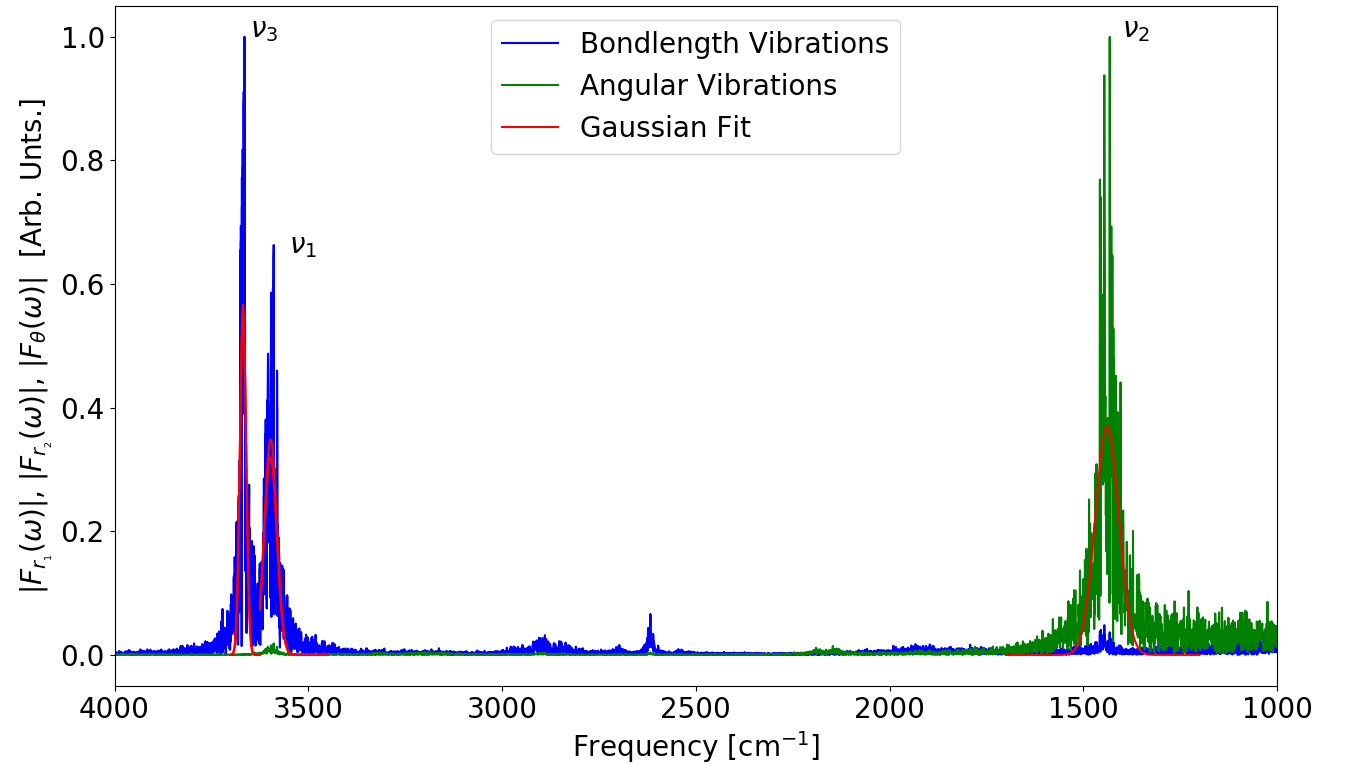
\includegraphics[scale=0.5]{images/Vibration_Modes.png}
			\caption{Normalized Fourier transforms for the O-H bond lengths and angle of a single water molecule in a Na montmorillonite simulation.}
			\label{fig:vib_modes}
		\end{figure}
		
		Figure~\ref{fig:vib_modes} depicts a resulting frequency spectrum. While the relative intensity between the $\nu_1$ and the $\nu_3$ modes is characteristic to their portions of the signal with respect to each other, the $\nu_2$ mode is calculated in such a way that one may not compare its intensity with that of the other two modes. It was possible to differentiate between the $\nu_1$ and $\nu_3$ modes by looking at the difference in their complex phases, which will be denoted as $\varphi(\omega)$.
		\begin{equation}
			\varphi(\omega) = \abs{\tan^{-1}\bigg( \frac{ \Im[F_{r_{_{1}}} (\omega)]}{\Re[F_{r_{_{1}}} (\omega)]} \bigg) - \tan^{-1}\bigg( \frac{ \Im[F_{r_{_{2}}} (\omega)]}{\Re[F_{r_{_{2}}} (\omega)]} \bigg)}
		\end{equation}
		When the frequencies appear in phase, their phase difference $\varphi$ should be near zero, while it should be approximately $\pi$ for two frequencies completely out of phase. Over the band at about 3700cm$^{-1}$, there was a phase difference of approximately $\pi$, while the phase difference in the band at 3550cm$^{-1}$ was approximately zero. One may see the plot of the phase difference in Figure~\ref{fig:phase} over this region.
		
		\begin{figure}
			\centering
			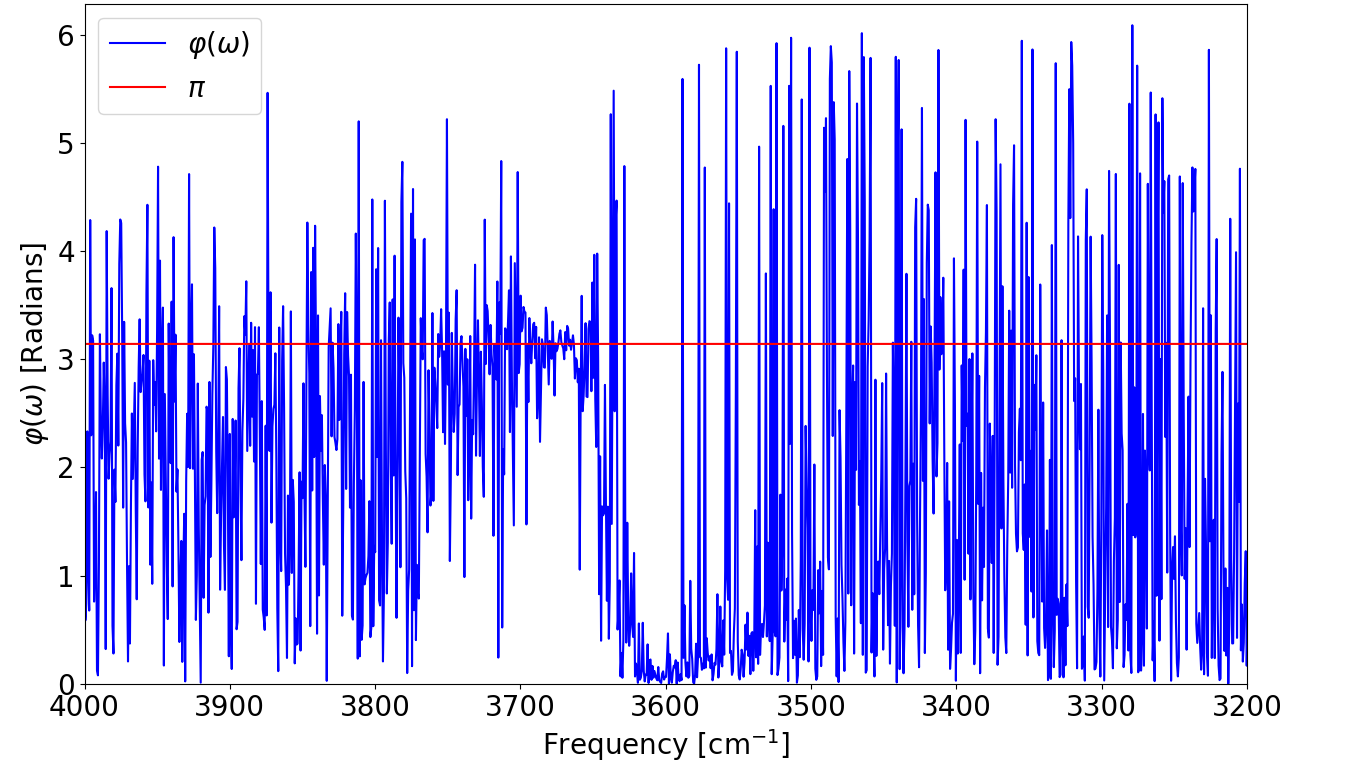
\includegraphics[scale=0.5]{images/phase.png}
			\caption{Phase difference in the Fourier transforms of the radial position of each hydrogen atom in the water molecule presented in Figure~\ref{fig:vib_modes}.}
			\label{fig:phase}
		\end{figure}
		
		For one simulation, the frequencies of the vibrational modes of each water molecule are determined, and then averaged over all molecules in the system.
	
	\section{Results}
		\subsection{ReaxFF Simulations}
		Reactions conducted using ReaxFF on one layer of kaolinite and one layer of water failed to relax appropriately. Even with the barostat and thermostat applied, large temperature and pressure oscillations were present. Upon visualizing the output in VMD, it was evident that the structure of the system degraded, and quickly lost any resemblance to the original structure. A solution to this problem was not found. It is possible that the force field used in this simulation was simply over parameterized to the system for which it was initially designed, or it was improperly implemented. Consequently, no data was collected using this method.
		
		\subsection{CVFF Simulations}
		The two models which were tested with the CVFF approach fared much better than the ReaxFF simulations. These models were able to maintain their structure, and relax to the prescribed 300K temperature. Slight oscillations in the pressure were observed; this is generally expected with large systems. The average frequencies for these two models are presented in Table~\ref{tab:frequencies}. Visualizations of the initial and final state of each system are provided in Figure~\ref{fig:na_visual} and Figure~\ref{fig:mont_visual}. The larger single layer of K montmorillonite appears to become two layers at the end, due to a rotation of the entire sheet within the simulation box, which is repeated due to the periodic boundary conditions. One may view the reported frequencies from the literature, and from this works experimental portions in Table~\ref{tab:frequency_comparison}. For both the $\nu_1$ and $\nu_2$ modes, the differences between the experimental and simulation frequencies are approximately 90$cm^{-1}$. It is possible that this is a constant difference in the model, but more trials and examinations will be required to see if this is the case.

		\begin{table}
			\centering
			\caption{Frequencies of water vibrational modes in CVFF simulations.}
			\label{tab:frequencies}
			\begin{tabular}{|c|c|}
			\hline
			\textbf{InterfaceFF Base Model} & \textbf{Average Frequencies} \\
			\hline
			\hline
			\multirow{3}{*}{mont0\_400\_Na\_15\_cell} & $\nu_1 = 3587 \pm 11\quad cm^{-1} $\\ & $\nu_2 = 1444 \pm 21 \quad cm^{-1}$ \\ & $\nu_3 = 3664 \pm \,\,\,6 \quad cm^{-1}$\\
			\hline
			\multirow{3}{*}{mont0\_333\_layer\_5nm\_neutral\_edges\_pH3} & $\nu_1 = 3588 \pm 12\quad cm^{-1} $\\ & $\nu_2 = 1443 \pm 26 \quad cm^{-1}$\\ & $\nu_3 = 3665 \pm \,\,\,6 \quad cm^{-1}$\\
			\hline
			\end{tabular}
		\end{table}

		\begin{table}
			\centering
			\caption{Frequencies obtained from literature and experimentation.}
			\label{tab:frequency_comparison}
			\begin{tabular}{|c|c|}
			\hline
			\rule{0pt}{2.5ex} \textbf{Frequencies From Madejova Baseline Study \cite{madejova2001baseline}} & \textbf{IR Experimental Results} \\
			\hline
			\hline
			\rule{0pt}{2.5ex} $\nu_1$ : 3373 - 3393 $cm^{-1}$ & $\nu_1$ : 3395 - 3420 $cm^{-1}$ \\
			\rule{0pt}{2.5ex} $\nu_2$ : 1629 - 1633 $cm^{-1}$ & $\nu_2$ : 1628 - 1630 $cm^{-1}$ \\
			\hline
			\end{tabular}
		\end{table}


		\begin{figure}
			\centering
			\begin{subfigure}{0.5\textwidth}
				\centering
				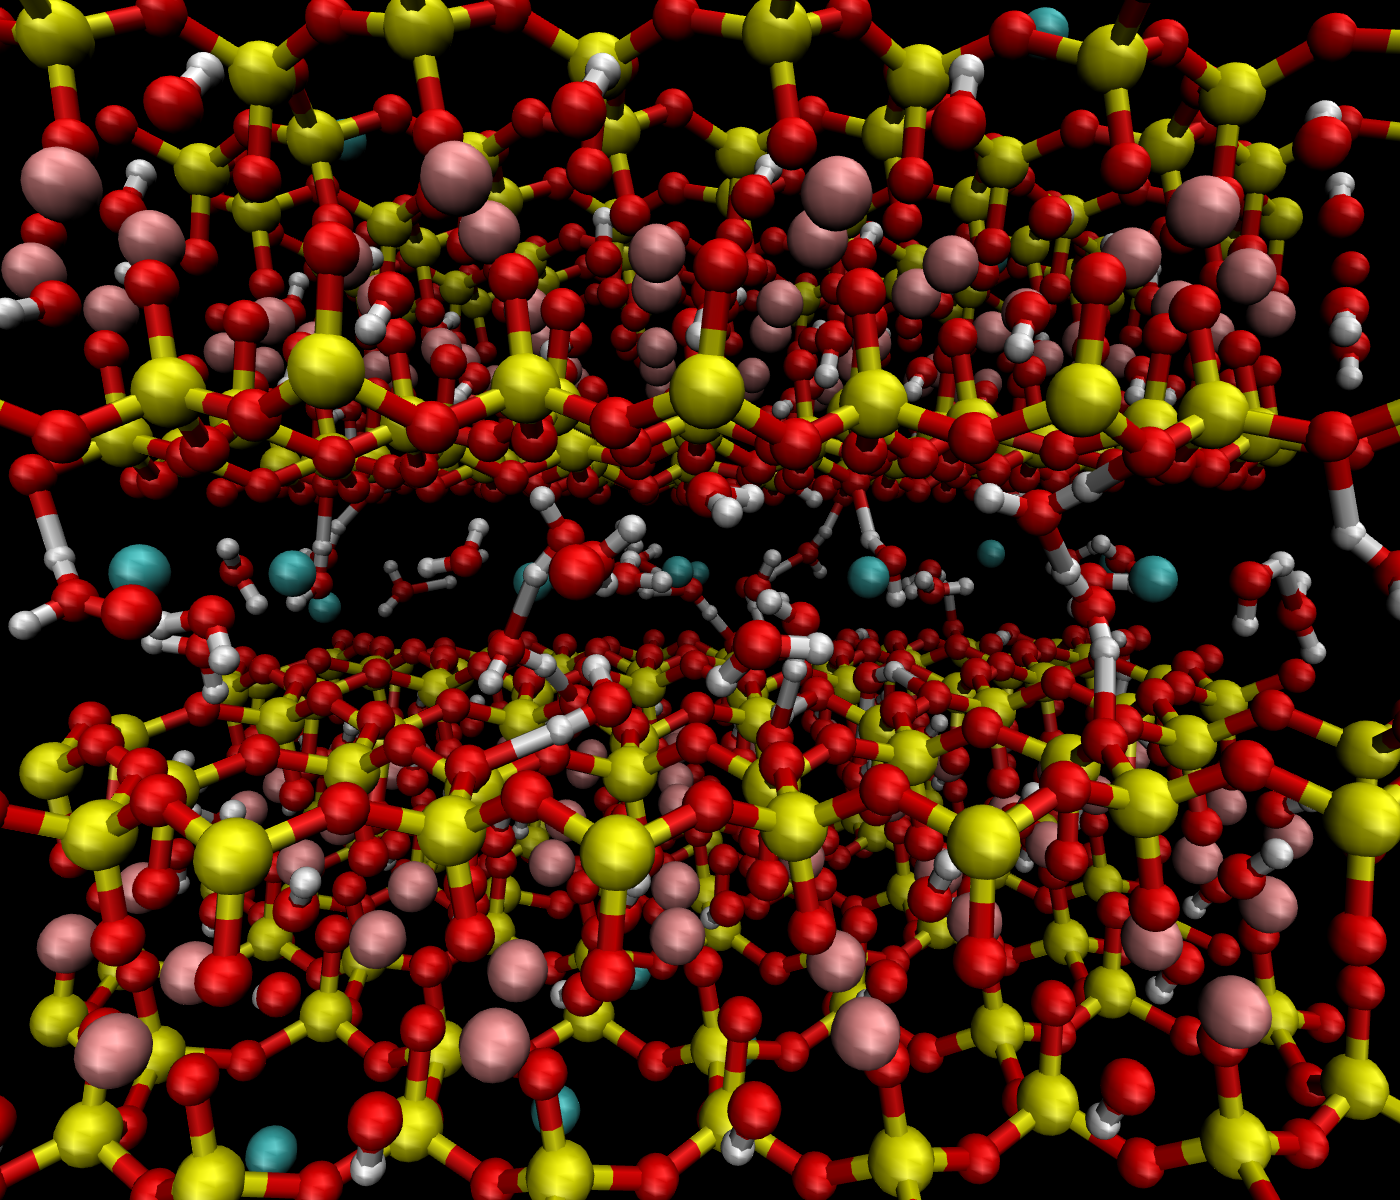
\includegraphics[scale=0.22]{images/na_init.png}
				\caption{Initial state}
			\end{subfigure}%
			\begin{subfigure}{0.5\textwidth}
				\centering
				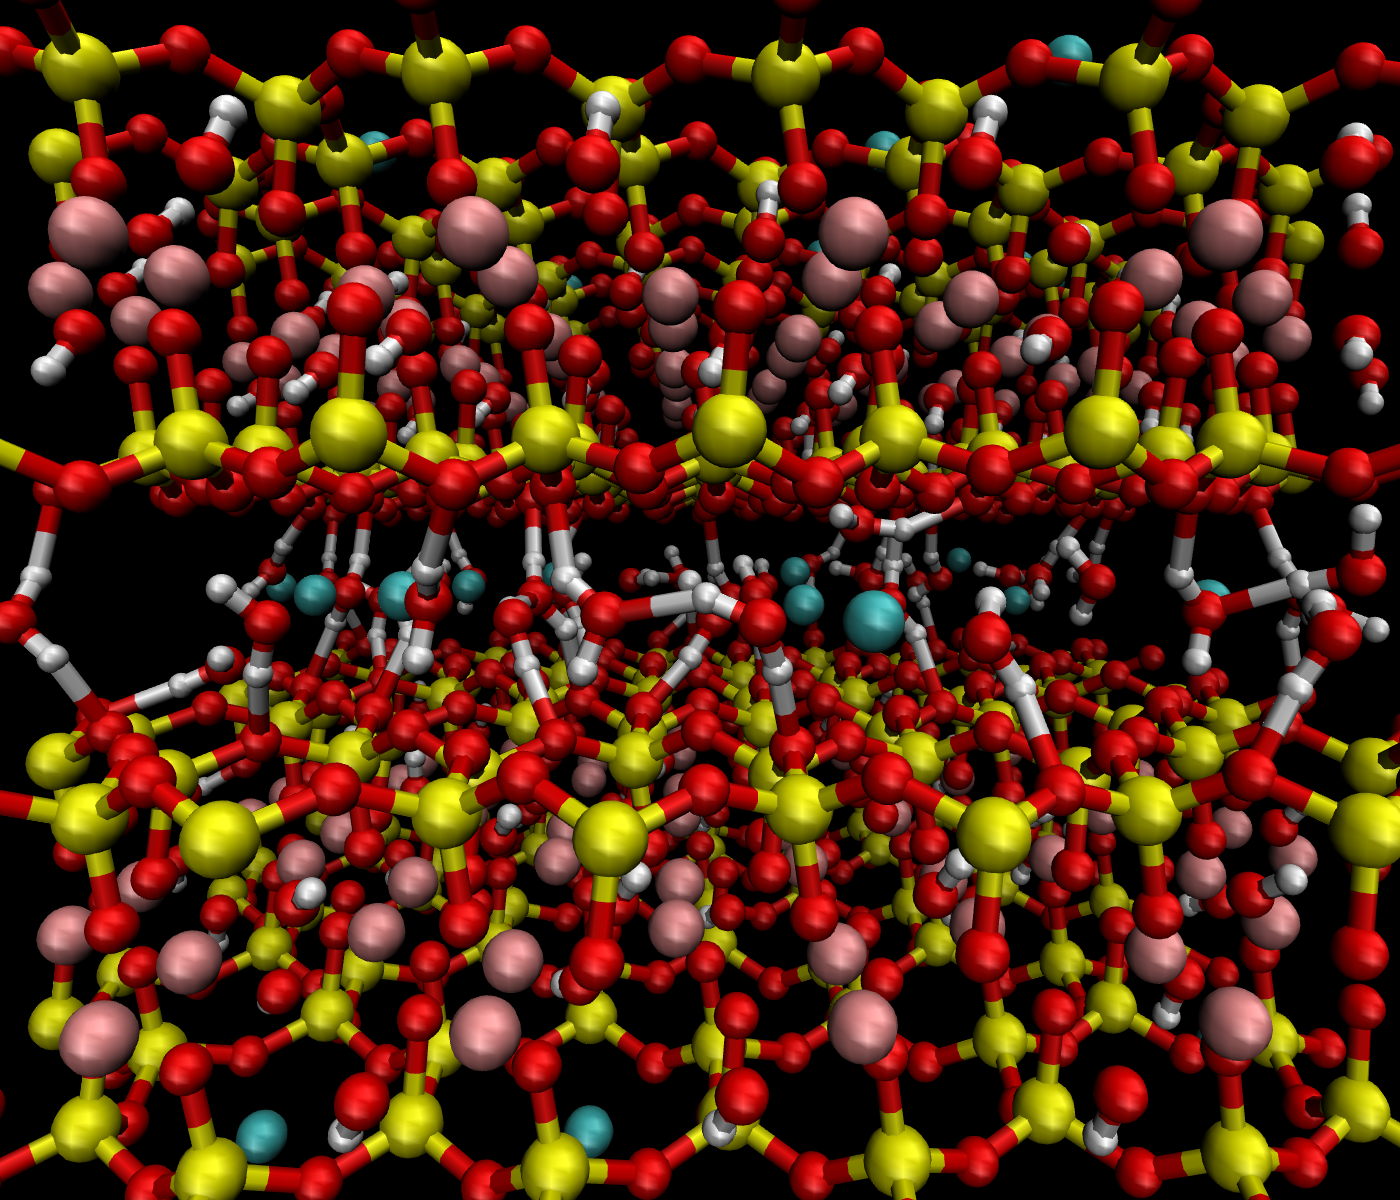
\includegraphics[scale=0.22]{images/na_fin.png}
				\caption{Final state}
			\end{subfigure}
			\caption{VMD Visualizations of Na montmorillonite cell simulation.}
			\label{fig:na_visual}
		\end{figure}
		
		\begin{figure}
			\centering
			\begin{subfigure}{0.5\textwidth}
				\centering
				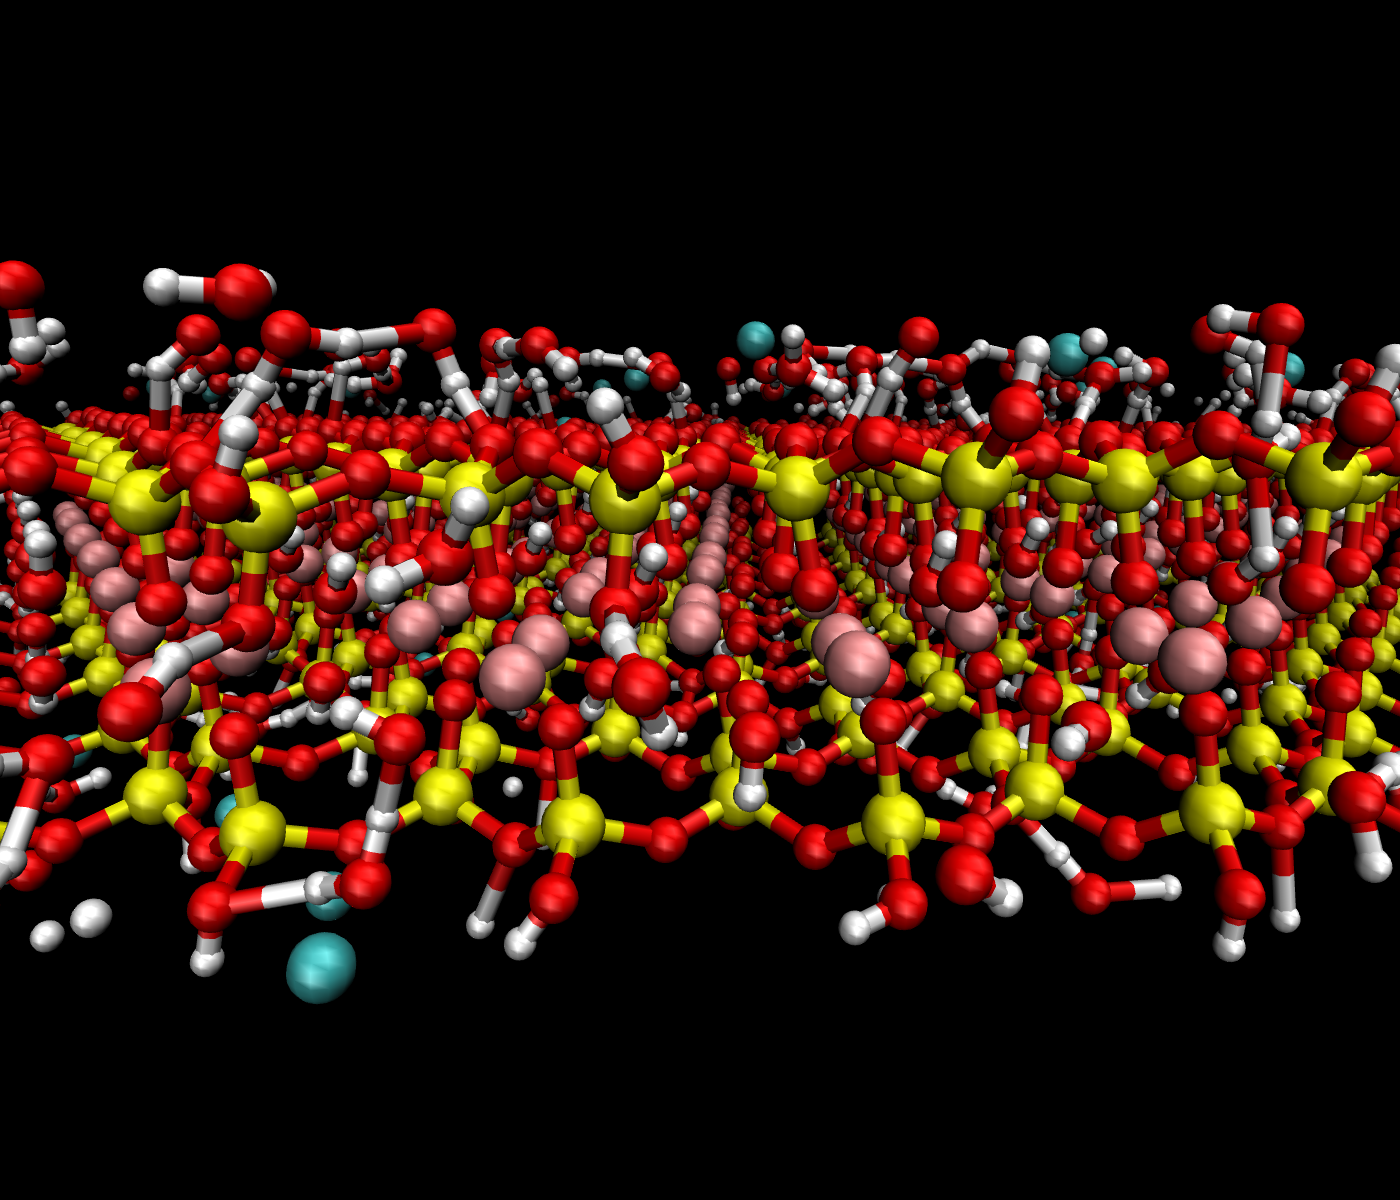
\includegraphics[scale=0.22]{images/mont_init.png}
				\caption{Initial state}
			\end{subfigure}%
			\begin{subfigure}{0.5\textwidth}
				\centering
				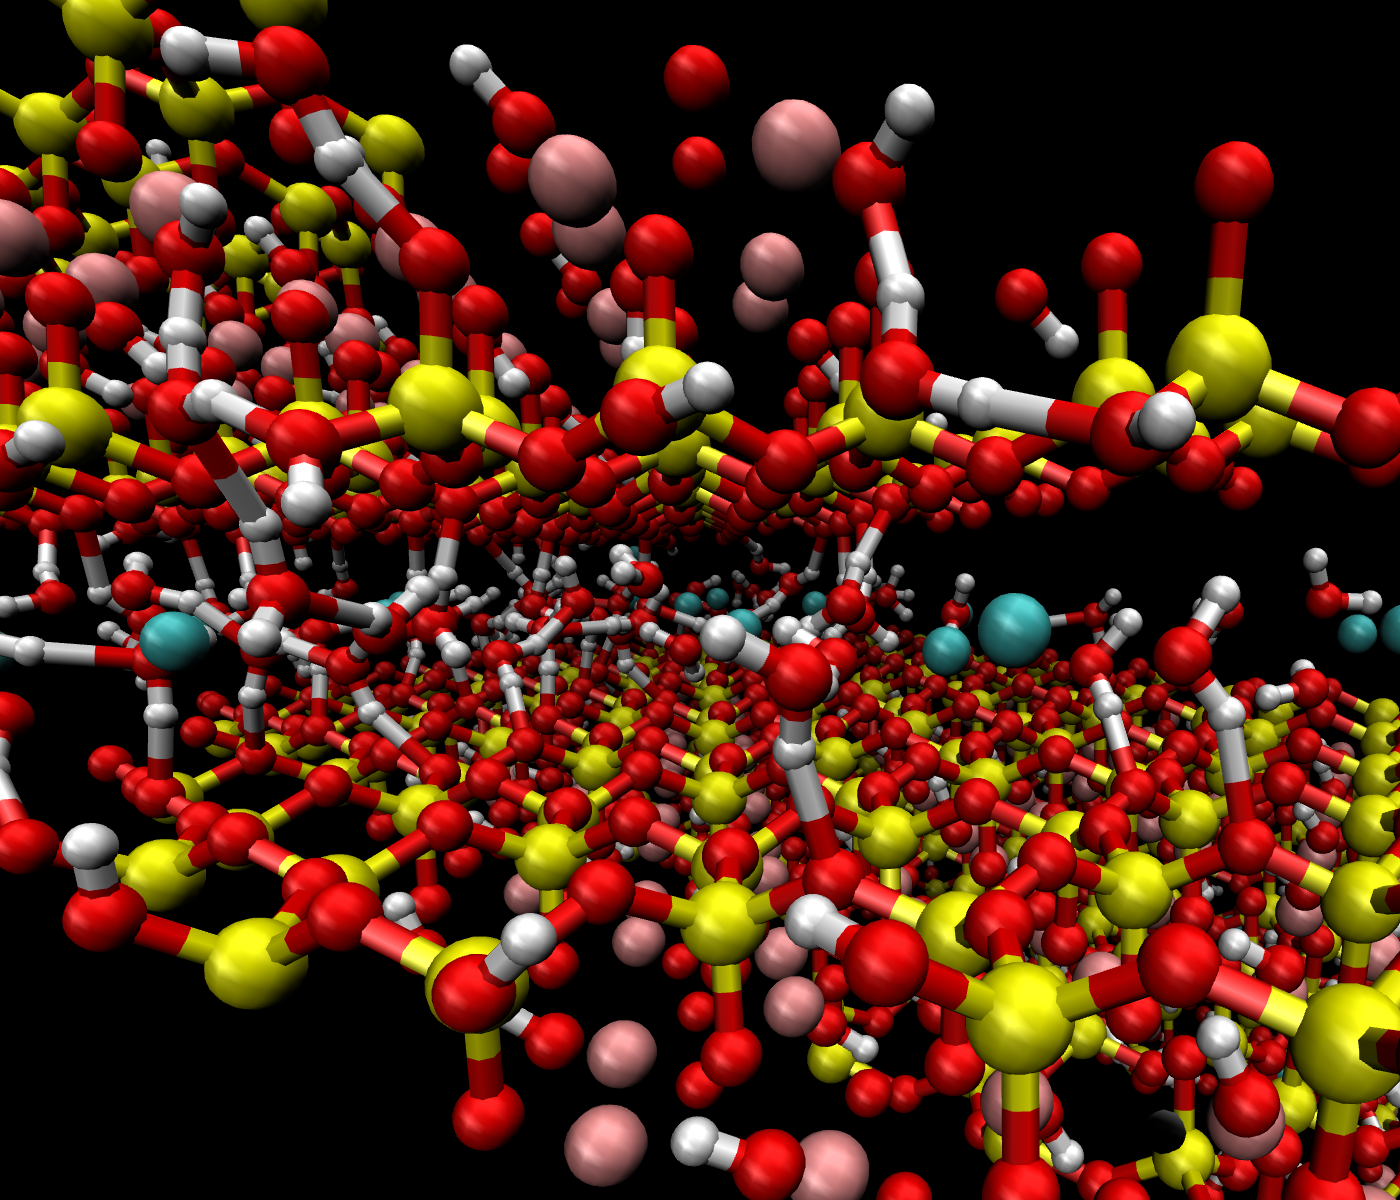
\includegraphics[scale=0.22]{images/mont_fin.png}
				\caption{Final state}
			\end{subfigure}
			\caption{VMD Visualizations of K montmorillonite sheet simulation.}
			\label{fig:mont_visual}
		\end{figure}
		
				
			
			


%%% Local Variables: 
%%% mode: latex
%%% TeX-master: t
%%% End: 